\documentclass{article}

\usepackage{hyperref}
\usepackage{graphicx}

\title{Api RESTful (REpresentational State Transfer)}
\author{Riccardo Cambianica}
\begin{document}
    \maketitle
     \newpage
     \tableofcontents
     \newpage
     \section{Cos'è un API?}
         Le API, acronimo di Application Programming Interface (interfaccia di programmazione delle applicazioni) sono un insieme di definizioni e protocolli con i quali vengono realizzati e integrati software applicativi. In altre parole, un'API facilita la comunicazione con il sistema che può così comprendere e soddisfare la richiesta. L'API funge quindi da elemento di intermediazione tra gli utenti o i clienti e le risorse o servizi web che questi intendono ottenere. È anche un mezzo con il quale un'organizzazione può condividere risorse e informazioni assicurando al contempo sicurezza, controllo e autenticazione, poiché stabilisce i criteri di accesso.
         \begin{figure}[htbp]
             \centering
             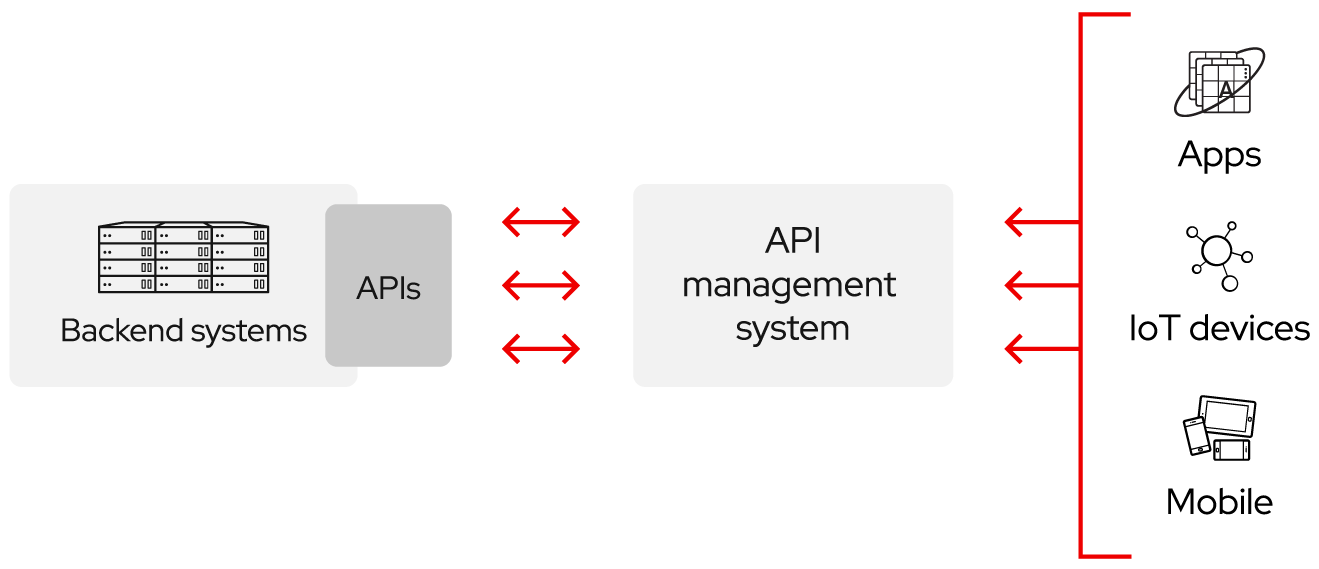
\includegraphics[width=0.85\textwidth]{pics/API-page-graphic.png}  
             \caption{Funzione e ruolo delle API}
             \label{fig:api}
         \end{figure}
     \section{REST}
        Un'API RESTful, è un'interfaccia di programmazione delle applicazioni (API o API web) conforme ai vincoli dello stile architetturale REST, che consente l'interazione con servizi web RESTful. E' bene fare una distinguo: REST non è un protocollo né uno standard.
        
        Affinché un'API sia considerata RESTful, deve rispettare i criteri indicati di seguito:
        \begin{itemize}
            \item Un'architettura client-server composta da client, server e risorse, con richieste gestite tramite HTTP.
            \item Una comunicazione client-server stateless, che quindi non prevede la memorizzazione delle informazioni del client tra le richieste Get; ogni richiesta è distinta e non connessa.
            \item Dati memorizzabili nella cache che ottimizzano le interazioni client-server.
            \item Un'interfaccia uniforme per i componenti, in modo che le informazioni vengano trasferite in una forma standard. Ciò impone che:
                \begin{itemize}
                    \item le risorse richieste siano identificabili e separate dalle rappresentazioni inviate al client;
                    \item le risorse possano essere manipolate dal client tramite la rappresentazione che ricevono poiché questa contiene le informazioni sufficienti alla manipolazione;
                    \item i messaggi \textbf{autodescrittivi} restituiti a un client contengano le informazioni necessarie per descrivere come il client deve elaborare l'informazione;
                    \item le informazioni siano ipermediali e ipertestuali, ovvero accedendo alla risorsa il client deve poter individuare, attraverso hyperlink, tutte le altre azioni disponibili al momento.
                \end{itemize}
            \item Un sistema su più livelli che organizza ogni tipo di server (ad esempio quelli responsabili della sicurezza, del bilanciamento del carico, ecc.) che si occupa di recuperare le informazioni richieste in gerarchie, invisibile al client.
            \item Codice on demand (facoltativo): la capacità di inviare codice eseguibile dal server al client quando richiesto, estendendo la funzionalità del client. 
        \end{itemize}

        Sebbene l'API REST debba essere conforme a questi criteri, il suo impiego è comunque considerato più semplice rispetto a quello di un protocollo prescrittivo come Anchor textSOAP (Simple Object Access Protocol), che presenta requisiti specifici come la messaggistica XML e la conformità integrata di sicurezza e transazioni, che lo rendono più lento e pesante. 
        Al contrario, REST è un insieme di linee guida applicabili quando necessario, il che rende le API REST più rapide, leggere e con una maggiore scalabilità, ottimali quindi per l'\textbf{Internet of Things (IoT)} e lo sviluppo di \textbf{app mobili}. 
    
\end{document}